\chapter{Hypothesis Tests}
\label{cha:hypothesis_tests}

\section{Testing Problems}%
\label{sec:testing_problems}

\textbf{Observation}: X, values in sample space
\(\mathcal{X} \subset \mathbb{R}^d\)

\textbf{Model:} \(\{P_{\theta} : \theta \in \Theta\}\) with parameter
space \(\Theta \subset \mathbb{R}^k\) .


A \textbf{testing problem} amounts to deciding between two competing hypotheses regarding the true parameter $\theta$:
\[
H_0: X \sim P_{\theta} \text{ with } \theta \in \Theta_0 \quad \text{versus} \quad H_1: X \sim P_{\theta} \text{ with } \theta \in \Theta_1,
\]
where $\Theta_0$ and $\Theta_1$ form a partition of the parameter space $\Theta$ (i.e., they are disjoint).

\subsubsection{The Action Space and Asymmetry}

The decision problem involves an action space $\mathcal{A} = \{0, 1\}$. While formally symmetric, the Neyman--Pearson theory (which we will cover later) adopts an \textbf{asymmetric view}:

\begin{itemize}
    \item $\bs{H_0}$ (\textbf{Null Hypothesis}): Represents the default scenario, status quo, or ``no effect."
    \item $\bs{H_1}$ (\textbf{Alternative Hypothesis}): Represents a discovery, a new effect, or a deviation from the norm.
\end{itemize}

Consequently, the actions are interpreted as:
\begin{itemize}
    \item $a = 0$: \textbf{Do not reject $H_0$.}
    \begin{itemize}
        \item This is \emph{not} a confirmation that $H_0$ is true.
        \item It is interpreted as a ``missed opportunity" to find a signal, which is generally considered less severe than a false discovery.
    \end{itemize}
    \item $a = 1$: \textbf{Reject $H_0$} (Accept $H_1$).
    \begin{itemize}
        \item This is a claim that the default assumption is false.
        \item Making this claim erroneously is considered ``something bad" (a false positive) and is strictly controlled.
    \end{itemize}
\end{itemize}

\begin{remark}[``\(p\)--value crisis" and Reproducibility]
In many scientific fields (e.g., medicine, psychology), there is a strong culture of supporting claims with statistical significance (\(p\)--values).
\begin{itemize}
    \item A rejection of $H_0$ (e.g., ``The drug does nothing") is often required to publish results.
    \item \textbf{Effect Size vs. Significance:} A significant result (tiny \(p\)--value) only tells us that $H_0$ is false; it does not tell us if the effect is \emph{meaningful}. A drug might statistically extend life by 1 second (rejecting ``no effect"), but this is clinically irrelevant. Modern statistics emphasizes reporting \textbf{confidence intervals} and \textbf{effect sizes} alongside tests to capture the magnitude of the benefit.
    \item \textbf{Replicability:} If a researcher repeats an experiment many times and only reports the one successful test (hiding the failures), the statistical guarantees of the test are invalidated. This ``file drawer problem" contributes to the replication crisis in science.
\end{itemize}

\end{remark}

\begin{ex}[Television ads and NBC Guidelines]\label{ex:television_ads}
The following requirements for television advertisements (based on historical NBC guidelines) illustrate how testing formulations change based on the claim being made.
\begin{enumerate}[label=\alph*)]
\item 

\textbf{Superiority Claim (``Product A is better than B")}
To air a commercial claiming superiority, NBC requires a study with $n \ge 300$ participants. Let $X \sim \text{Binomial}(n,\theta)$ be the count of participants preferring A.
The null hypothesis must represent the opposite of the claim (i.e., A is not better).
\[
H_0: \theta \le 0.5 \quad \text{vs.} \quad H_1: \theta > 0.5
\]
The claim is allowed only if the test rejects $H_0$ at a 95\% confidence level.

\item 
\textbf{Parity Claim (``Product A is as good as B")}
To claim parity, the requirements are stricter ($n \ge 500$). If the observed preference rate $X/n < 0.5$, the claim is allowed only if we \textbf{fail to reject} the hypothesis of equality:
\[
H_0: \theta = 0.5 \quad \text{vs.} \quad H_1: \theta \neq 0.5
\]
at a 90\% confidence level.
\end{enumerate}

\textbf{Discussion on ``Gaming" the System:}
In practice, a company might conduct a study for Scenario A and fail to reject $H_0$. If they simply discard that study and repeat the experiment until they get a ``lucky" rejection (without telling the network about the failures), they are exploiting random chance. This highlights the importance of pre-registration in clinical trials (e.g., FDA requirements for vaccines) to prevent such ``\(p\)--hacking."

\end{ex}

\subsection{Tests and Their Errors}

\begin{definition}[Non-randomized test]
A \textbf{non-randomized test} is a decision rule \(d: \mathcal{X} \to \{0,1\}\).
\begin{itemize}
    \item The value \(d(x) = 1\) corresponds to rejecting \(H_0\) (accepting \(H_1\)).
    \item The value \(d(x) = 0\) corresponds to accepting \(H_0\) (rejecting \(H_1\)).
\end{itemize}
The \textbf{rejection region} is the set of observations leading to rejection:
\[ S_1 = \{x \in \mathcal{X} : d(x) = 1\}. \]
The \textbf{acceptance region} is its complement \(\mathcal{X} \setminus S_1\).
\end{definition}



\subsubsection{Type I and Type II Errors}
In this binary decision framework, there are two specific ways to make an incorrect decision. While other fields use descriptive terms like ``False Positive" (Sensitivity/Specificity), statistics traditionally uses the labels Type I and Type II.

\begin{itemize}
    \item \textbf{Type I error (False Positive):} Rejecting \(H_0\) when it is actually true (\(\theta \in \Theta_0\)).
    \item \textbf{Type II error (False Negative):} Accepting \(H_0\) when it is actually false (\(\theta \in \Theta_1\)).
\end{itemize}

\subsubsection{Randomized Tests}
It is often mathematically convenient to allow \textbf{randomized decision rules}. In practice, you typically want a clear ``Yes/No" answer, but allowing a test to output a \textit{probability} of rejection simplifies the theoretical search for optimal tests (see convexity below).

\begin{definition}[Randomized Test]
    \leavevmode
\begin{enumerate}
    \item[(i)] A \textbf{randomized decision rule} maps observed values \(x\) to probability distributions on the action space \(\mathcal{A}\).
    \item[(ii)] A \textbf{randomized test} is a function \(d: \mathcal{X} \to [0,1]\), where \(d(x)\) represents the probability of rejecting \(H_0\) given observation \(x\).
\end{enumerate}
In the sequel, the term ``test'' will generally refer to randomized tests, with non-randomized tests being the special case where \(d(x) \in \{0, 1\}\).
\end{definition}

\begin{remark}[Convexity]
The set of randomized tests is \textbf{convex}.
If \(d_1\) and \(d_2\) are tests (mapping into \([0,1]\)) and \(\alpha \in [0,1]\), then the convex combination
\[ d_{\text{new}}(x) = \alpha d_1(x) + (1-\alpha) d_2(x) \]
is also a valid test, as the output remains in \([0,1]\). This property is crucial for optimization theory in hypothesis testing.
\end{remark}

\subsection{Neyman--Pearson Loss and Risk of Tests}

To apply decision theory to hypothesis testing, we define a loss function that penalizes incorrect decisions. The \textbf{Neyman--Pearson (NP) loss} is the natural choice for the binary action space $\mathcal{A} = \{0, 1\}$. It focuses solely on whether the decision matches the truth state of $\theta$.

\subsubsection{The Loss Function}

Let $c_1 > 0$ be the cost of a Type I error and $c_0 > 0$ be the cost of a Type II error.

\begin{definition}[Neyman-Pearson Loss]
The loss function $L(\theta, a)$ for a deterministic action $a \in \{0, 1\}$ is defined as:

\begin{center}
\begin{tabular}{l|c|c}
\toprule
\textbf{State of Nature (\(L(\theta,a)\))} & \textbf{Accept $H_0$ ($a=0$)} & \textbf{Reject $H_0$ ($a=1$)} \\
\midrule
$H_0$ True ($\theta \in \Theta_0$) & 0 & $c_1$ \\
$H_1$ True ($\theta \in \Theta_1$) & $c_0$ & 0 \\
Indifferent ($\theta \notin \Theta_0 \cup \Theta_1$) & 0 & 0 \\
\bottomrule
\end{tabular}
\end{center}
\end{definition}

\paragraph{Extension to Randomized Tests}
As discussed previously, a randomized test outputs a probability $p = d(x) \in [0,1]$ rather than a strict action. To define the loss for a probability $p$, we consider the \textbf{expected loss} over the internal randomization of the test.

Let $A \sim \text{Bernoulli}(p)$ be the random action generated by the test. The extended loss function $L: \Theta \times [0,1] \to \mathbb{R}$ is:
\[
L(\theta, p) = \mathsf{E}_{A \sim \text{Bernoulli}(p)}[L(\theta, A)] = p L(\theta, 1) + (1 - p) L(\theta, 0).
\]
Substituting the values from the NP table, this simplifies to a linear function of $p$:
\[
L(\theta, p) = 
\begin{cases} 
p \cdot c_1 & \text{if } \theta \in \Theta_0 \\
(1 - p) \cdot c_0 & \text{if } \theta \in \Theta_1
\end{cases}
\]
Intuitively, if the Null is true ($\theta \in \Theta_0$), the ``mistake" is rejecting it (action 1). You pay the cost $c_1$ weighted by the probability $p$ that you actually make that mistake.

\subsubsection{The Risk Function}

The risk $R(\theta, d)$ is the expected loss over the randomness of the data $X$.

\[
R(\theta, d) = \mathsf{E}_{\theta} \big[ L(\theta, d(X)) \big].
\]

Using the linearity of the expectation, we can express the risk directly in terms of the test's behavior.

\paragraph{For a Non-Randomized Test ($d(X) \in \{0,1\}$):}
\[
R(\theta, d) = 
\begin{cases} 
c_1 \cdot \mathsf{P}_{\theta}(d(X) = 1) & \text{if } \theta \in \Theta_0, \\ 
c_0 \cdot \mathsf{P}_{\theta}(d(X) = 0) & \text{if } \theta \in \Theta_1. 
\end{cases}
\]

\paragraph{For a Randomized Test ($d(X) \in [0,1]$):}
Since $\mathsf{E}_{\theta}[d(X)]$ represents the expected probability of rejection:
\[
R(\theta, d) = 
\begin{cases} 
c_1 \cdot \mathsf{E}_{\theta}[d(X)] & \text{if } \theta \in \Theta_0, \\ 
c_0 \cdot (1 - \mathsf{E}_{\theta}[d(X)]) & \text{if } \theta \in \Theta_1. 
\end{cases}
\]

\subsubsection{The Power Function}

Notice that in both cases above, the risk is entirely determined by a single quantity: the expected value of the test function.

\begin{definition}[Power Function]
The \textbf{power function} of a test $d$, denoted $\beta_d(\theta)$ (or simply $\beta(\theta)$), is the probability (or expected probability) of rejecting the null hypothesis as a function of $\theta$:
\[
\beta_d(\theta) := \mathsf{E}_{\theta}[d(X)].
\]
\end{definition}



This definition unifies both cases:
\begin{itemize}
    \item If $d$ is non--randomized, $\mathsf{E}_{\theta}[d(X)] = 1 \cdot \mathsf{P}(d(X)=1) + 0 = \mathsf{P}_{\theta}(\text{Reject } H_0)$.
    \item If $d$ is randomized, it is the average rejection probability.
\end{itemize}

\textbf{Relationship between Risk and Power:}
We can now rewrite the risk compactly using the power function:
\[
R(\theta, d) = 
\begin{cases} 
c_1 \beta(\theta) & \text{if } \theta \in \Theta_0 \quad \text{(Type I Error Risk)} \\ 
c_0 (1 - \beta(\theta)) & \text{if } \theta \in \Theta_1 \quad \text{(Type II Error Risk)}
\end{cases}
\]
Thus, characterizing the performance of a test is equivalent to studying its power function. Ideally, we want $\beta(\theta) \approx 0$ for $\theta \in \Theta_0$ and $\beta(\theta) \approx 1$ for $\theta \in \Theta_1$.

\subsection{Tests in Neyman-Pearson Form}
\label{sec:tests_np_form}

In practice, we rarely construct arbitrary randomized mappings from $\mathcal{X}$ to $[0,1]$. Instead, nearly all practical tests follow the specific \textbf{Neyman-Pearson form} (or ``0-1 form''). This structure reduces the dimensionality of the data to a single scalar and applies a threshold.

\begin{definition}[Neyman-Pearson Form]
A test $d$ is in Neyman-Pearson form if it is defined by a \textbf{test statistic} $T: \mathcal{X} \to \mathbb{R}$, a \textbf{critical value} $k \in \mathbb{R}$, and a randomization constant $\gamma \in [0,1]$ such that:

\[
d(x) = \begin{cases} 
1 & \text{if } T(x) > k, \\ 
\gamma & \text{if } T(x) = k, \\ 
0 & \text{if } T(x) < k. 
\end{cases}
\]
\end{definition}



\subsubsection{Intuition and Components}

\begin{itemize}
    \item \textbf{The Test Statistic \(T(x)\):} This function summarizes the complex dataset (e.g., a vector of observations) into a single number relevant to the hypothesis. 
    \begin{itemize}
        \item We choose \(T\) such that it tends to take \textbf{small to moderate values} when \(H_0\) is true.
        \item It tends to take \textbf{large values} when \(H_0\) is false (i.e., when \(H_1\) is true).
    \end{itemize}
    
    \item \textbf{The Critical Value \(k\):} This is the threshold of evidence. If the signal \(T(x)\) exceeds \(k\), we reject \(H_0\). The ``art'' of designing a statistical test lies in calibrating this \(k\) to achieve a specific risk profile (e.g., ensuring the Type I error probability does not exceed 5\%).

    \item \textbf{The Randomization \(\gamma\):} If the statistic lands exactly on the threshold (\(T(x) = k\)), we may need ``wiggle room'' to satisfy strict error constraints. In this boundary case, we flip a coin with probability \(\gamma\) to decide whether to reject. (Note: For continuous data, \(P(T(X)=k) = 0\), so \(\gamma\) is often irrelevant).
\end{itemize}

\begin{ex}[Application to Television Ads]
Revisiting \autoref{ex:television_ads} (Television ads), we can define the components as follows:

\begin{itemize}
    \item \textbf{Data:} The raw data might be a spreadsheet of $n$ rows, where each entry is a preference for Product A (1) or Product B (0).
    \item \textbf{Test Statistic:} We choose \(T(x) = \sum x_i\) (the total count of participants preferring A).
    \item \textbf{Logic:}
    \begin{itemize}
        \item If \(H_0\) is true (Product A is not better), we expect \(T(x)\) to be around \(n/2\) or lower.
        \item If \(H_1\) is true (Product A is better), we expect \(T(x)\) to be significantly higher.
    \end{itemize}
    \item \textbf{Decision:} We calculate a threshold \(k\) based on the Binomial distribution. If the count \(T(x) > k\), we reject \(H_0\) and air the ad.
\end{itemize}
\end{ex}

\subsection{Bayes Tests}
\label{sec:bayes_tests}

In the Bayesian framework, we treat the parameter $\theta$ as a random variable.
Let $\Pi$ be a \textbf{Prior distribution} on the parameter space, which is partitioned into $\Theta = \Theta_0 \dot{\cup} \Theta_1$. Let $\Pi(\cdot|x)$ denote the posterior distribution given the data $x \in \mathcal{X}$.

\subsubsection{Minimizing Posterior Risk}
Unlike the frequentist risk (which averages over data for a fixed $\theta$), the Bayesian approach fixes the data $x$ and averages the loss over the uncertainty in $\theta$ (the posterior).



Under the Neyman-Pearson (NP) loss structure (defined in the previous section), the \textbf{posterior risk} of taking a randomized action $p \in [0, 1]$ (where $p$ is the probability of rejecting $H_0$) is:

\[
\begin{split} 
\ell(x,p) &= \int_{\Theta} L(\theta,p) \; d\Pi(\theta|x) \\ 
&= \int_{\Theta_0} \underbrace{c_1 p}_{\text{Loss if } H_0 \text{ true}} \; d\Pi(\theta|x) + \int_{\Theta_1} \underbrace{c_0 (1-p)}_{\text{Loss if } H_1 \text{ true}} \; d\Pi(\theta|x) \\ 
&= p \cdot c_1 \cdot \Pi(\Theta_0|x) + (1-p) \cdot c_0 \cdot \Pi(\Theta_1|x).
\end{split}
\]

Rearranging terms to group by $p$:
\[
\ell(x,p) = p \left[ c_1 \Pi(\Theta_0|x) - c_0 \Pi(\Theta_1|x) \right] + c_0 \Pi(\Theta_1|x).
\]

\textbf{Optimization:}
A \textbf{Bayes test} (or Bayes rule) is the decision rule $d(x)$ that minimizes this posterior risk for every $x$:
\[ d(x) = \arg\min_{p \in [0,1]} \ell(x, p). \]

Note that $\ell(x, p)$ is a \textbf{linear function} of $p$ on the interval $[0,1]$.
\begin{itemize}
    \item If the slope (term in brackets) is negative, the minimum is at $p=1$.
    \item If the slope is positive, the minimum is at $p=0$.
    \item If the slope is zero, any $p$ works (the risks are balanced).
\end{itemize}



\begin{theo}[Bayes Test Form]
\label{thm:bayes_test_form}
A Bayes test under Neyman-Pearson loss has the form:
\[
d(x) = \begin{cases} 
1, & \text{if } c_0 \Pi(\Theta_1|x) > c_1 \Pi(\Theta_0|x), \\ 
\gamma(x), & \text{if } c_0 \Pi(\Theta_1|x) = c_1 \Pi(\Theta_0|x), \\ 
0, & \text{if } c_0 \Pi(\Theta_1|x) < c_1 \Pi(\Theta_0|x), 
\end{cases}
\]
where $\gamma(x) \in [0,1]$ is arbitrary.
\end{theo}

\subsubsection{Bayes Tests of Simple Hypotheses}
Consider the specific case where we compare exactly two distributions (Simple vs. Simple).
Let $\Theta_0 = \{\theta_0\}$ and $\Theta_1 = \{\theta_1\}$.
\begin{itemize}
    \item \textbf{Model:} $\mathsf{P}_{\theta_0}$ has density $p_0(x)$ and $\mathsf{P}_{\theta_1}$ has density $p_1(x)$.
    \item \textbf{Priors:} Let $\pi_0 := \Pi(\Theta_0)$ and $\pi_1 := \Pi(\Theta_1)$ with $\pi_0 + \pi_1 = 1$.
\end{itemize}

Using Bayes' theorem, the posterior probabilities are:
\[
\Pi(\Theta_0|x) = \frac{\pi_0 p_0(x)}{\pi_0 p_0(x) + \pi_1 p_1(x)}, \qquad \Pi(\Theta_1|x) = \frac{\pi_1 p_1(x)}{\pi_0 p_0(x) + \pi_1 p_1(x)}.
\]

Substituting these into \autoref{thm:bayes_test_form}, the denominators cancel out. We reject $H_0$ (action $d(x)=1$) if:
\[ c_0 \pi_1 p_1(x) > c_1 \pi_0 p_0(x). \]

\subsubsection{The Likelihood Ratio Test}
We can rearrange the inequality above to separate the data from the external factors (costs and priors). The Bayes test rejects $H_0$ when:

\[
\underbrace{\frac{p_1(x)}{p_0(x)}}_{\text{Likelihood Ratio}} > \underbrace{\frac{c_1}{c_0}}_{\text{Cost Ratio}} \cdot \underbrace{\frac{\pi_0}{\pi_1}}_{\text{Prior Odds}}
\]



\textbf{Interpretation:}
\begin{itemize}
    \item \textbf{Likelihood Ratio ($p_1/p_0$):} This quantifies how much more likely the observed data $x$ is under $H_1$ compared to $H_0$. It is the sufficient statistic for this problem.
    \item \textbf{Cost Ratio ($c_1/c_0$):} Adjusts the threshold based on consequences. If Type I errors are very expensive ($c_1$ is high), the threshold increases, requiring stronger evidence to reject.
    \item \textbf{Prior Odds ($\pi_0/\pi_1$):} Adjusts based on prior belief. If $H_0$ is extremely likely a priori (e.g., ``Trump will not win" in the lecturer's 2016 example), $\pi_0$ is high, pushing the threshold up.
\end{itemize}

\begin{remark}
If costs are equal ($c_1=c_0$) and priors are equal ($\pi_0=\pi_1$), the test simply compares which density is higher: reject if $p_1(x) > p_0(x)$.
\end{remark}

\begin{ex}[Testing Binomial Probability]
\label{ex:testing_binomial_prob}

Consider the test of a simple null hypothesis against a composite alternative:
\[
H_0: \theta = \theta_0 \quad \text{versus} \quad H_1: \theta \neq \theta_0,
\]
where the data follows a Binomial distribution, \(X \sim \text{Binomial}(n, \theta)\), with density:
\[
p_{\theta}(x) = \binom{n}{x} \theta^x (1-\theta)^{n-x}, \quad x = 0, 1, \dots, n.
\]

\paragraph{Constructing the Prior}
To construct a Bayes test, we must assign a prior distribution \(\Pi\) over \(\Theta = [0, 1]\). 

\begin{note}[Prior Selection]
    A continuous prior (e.g., \(\theta \sim \text{Uniform}[0,1]\)) would be inappropriate here because it assigns zero probability to any single point, meaning \(\Pi(\{\theta_0\}) = 0\). \emph{If the prior probability of \(H_0\) is zero, the posterior probability will also be zero regardless of the data. }
\end{note}

Therefore, we must assign a \textbf{positive probability mass} to \(\theta_0\). We define the prior as a mixture:
\[
\Pi = \pi_0 \cdot \delta_{\theta_0} + (1 - \pi_0) \cdot \text{Beta}(a, b),
\]
where \(\pi_0 \in (0, 1)\) is the prior probability that \(H_0\) is true, and \(\delta_{\theta_0}\) is a point mass (Dirac delta) at \(\theta_0\).



\paragraph{The Two-Stage Draw}
We can think of drawing a parameter \(\theta\) from this prior as a two-step random process:
\begin{enumerate}
    \item \textbf{Hypothesis Selection:} Flip a biased coin that shows Heads with probability \(\pi_0\).
    \item \textbf{Parameter Assignment:}
    \begin{itemize}
        \item If Heads (\(H_0\)): Set \(\theta = \theta_0\) (the coin is ``fair'' or fixed).
        \item If Tails (\(H_1\)): Draw \(\theta\) randomly from the alternative distribution, \(\theta \sim \text{Beta}(a, b)\).
    \end{itemize}
\end{enumerate}

\paragraph{Prior Predictive Probability}
To compute the posterior, we first need the marginal likelihood (prior predictive probability) of observing the data \(x\). By the Law of Total Probability, we integrate the likelihood against the prior mixture:

\[
\begin{split} 
\mathsf{P}(X=x) &= \int p_{\theta}(x) \; \mathrm{d}\Pi(\theta) \\ 
&= \pi_0 \underbrace{\int p_{\theta}(x) \; \mathrm{d}\delta_{\theta_0}(\theta)}_{\text{Likelihood under } H_0} + (1-\pi_0) \underbrace{\int p_{\theta}(x) \; \mathrm{d}\mathrm{Beta}(a,b)}_{\text{Likelihood under } H_1}.
\end{split}
\]

The first integral is simply the evaluation at the point mass. The second integral exploits the conjugacy of the Beta distribution with the Binomial likelihood (``lazy integration''):

\[
\begin{split}
\mathsf{P}(X=x) &= \pi_0 p_{\theta_0}(x) + (1-\pi_0) \frac{\Gamma(a+b)}{\Gamma(a)\Gamma(b)} \binom{n}{x} \int_0^1 \theta^{x+a-1} (1-\theta)^{n-x+b-1} \; \mathrm{d}\theta \\ 
&= \pi_0 \binom{n}{x} \theta_0^x (1-\theta_0)^{n-x} + (1-\pi_0) \binom{n}{x} \frac{\Gamma(a+b)}{\Gamma(a)\Gamma(b)} \frac{\Gamma(x+a)\Gamma(n-x+b)}{\Gamma(n+a+b)}. 
\end{split}
\]

\paragraph{Posterior Probability and Decision}
The posterior probability of the null hypothesis \(\Theta_0 = \{\theta_0\}\) is given by Bayes' Rule:

\[
\Pi(\Theta_0|x) = \frac{\mathsf{P}(X = x | \theta = \theta_0) \, \mathsf{P}(\theta = \theta_0)}{\mathsf{P}(X = x)} 
= \frac{\pi_0\binom{n}{x}\theta_0^x (1 - \theta_0)^{n-x}}{\mathsf{P}(X = x)}.
\]

The posterior for the alternative is simply the complement, \(\Pi(\Theta_1|x)=1-\Pi(\Theta_0|x)\).

A Bayes test under Neyman-Pearson loss compares the ratio of these posterior probabilities (the posterior odds) against the cost ratio:
\[
\text{Reject } H_0 \iff \frac{\Pi(\Theta_1|x)}{\Pi(\Theta_0|x)} > \frac{c_1}{c_0}.
\]

\end{ex}

\section{Most Powerful Tests}
\label{sec:most_powerful_tests}

In the previous sections on Decision Theory and Bayes tests, we assumed we could quantify the loss of making errors (via costs $c_0, c_1$) and potentially assign prior probabilities. In practice, however, these values are often unknown or controversial (e.g., what is the exact cost of a medical side effect versus a cure?).

\subsubsection{The Neyman-Pearson Approach}
The Neyman-Pearson (NP) framework avoids assigning specific costs by treating the hypotheses asymmetrically. 
\begin{itemize}
    \item \textbf{Null Hypothesis ($H_0$):} Represents the status quo, current scientific standard, or ``no effect."
    \item \textbf{Alternative Hypothesis ($H_1$):} Represents a new discovery, effect, or change.
\end{itemize}

We consider rejecting $H_0$ when it is true (Type I Error) to be the ``worse" mistake. Therefore, we impose a strict constraint on this error probability.

%\subsubsection{Definitions and Setup}

\begin{definition}[Significance Level]
We require a test $d(X)$ to have a \textbf{significance level} $\alpha \in (0, 1)$. This means the probability of rejecting $H_0$ when it is true is bounded by $\alpha$:
\[
\mathsf{E}_{\theta}[d(X)] \le \alpha, \quad \forall \theta \in \Theta_0.
\]
Commonly, $\alpha = 0.05$ (a convention popularized by Fisher).
\end{definition}



Subject to this constraint, we seek to maximize the test's ability to detect the alternative.

\begin{definition}[Power]
The \textbf{power} of a test is the probability of correctly rejecting $H_0$ when $H_1$ is true:
\[
\beta(\theta) = \mathsf{E}_{\theta}[d(X)] \quad \text{for } \theta \in \Theta_1.
\]
\end{definition}

\subsubsection{Most Powerful (MP) Tests for Simple Hypotheses}

Consider the simplest case where we test two simple hypotheses:
\[ \Theta_0 = \{\theta_0\} \quad \text{and} \quad \Theta_1 = \{\theta_1\}. \]

\begin{definition}[Most Powerful Test]
A test $d$ is a \textbf{Most Powerful (MP) level $\alpha$ test} if:
\begin{enumerate}%[label=\roman*)]
    \item \textbf{Constraint:} It satisfies the size constraint:
    \[ \mathsf{E}_{\theta_0}[d(X)] \leq \alpha. \]
    \item \textbf{Maximization:} For any other test $d'$ that satisfies the size constraint, $d$ has greater or equal power:
    \[ \mathsf{E}_{\theta_1}[d(X)] \geq \mathsf{E}_{\theta_1}[d'(X)]. \]
\end{enumerate}
\end{definition}

\begin{remark}[Existence of Densities]
    
To derive these tests, we typically work with probability densities $p_0$ and $p_1$ corresponding to $\mathsf{P}_{\theta_0}$ and $\mathsf{P}_{\theta_1}$.

     Assuming the existence of these densities is \textbf{not} a restrictive assumption.

     Even if $\mathsf{P}_{\theta_0}$ and $\mathsf{P}_{\theta_1}$ are singular with respect to Lebesgue measure (or discrete), we can always define a dominating measure $\nu = \mathsf{P}_{\theta_0} + \mathsf{P}_{\theta_1}$.

     By the Radon--Nikodym theorem, densities $p_0 = \frac{dP_{\theta_0}}{d\nu}$ and $p_1 = \frac{dP_{\theta_1}}{d\nu}$ always exist.
\end{remark}

\subsubsection{The Neyman-Pearson Lemma}
\label{sec:neyman_pearson_lemma}

\begin{theo}[Neyman-Pearson Lemma, 
    Lehmann and Romano 2005, Theorem 3.2.1]
\label{thm:neyman_pearson}

Consider testing a simple null hypothesis against a simple alternative:
\[ H_0: \theta = \theta_0 \quad \text{vs.} \quad H_1: \theta = \theta_1. \]
Let $p_0$ and $p_1$ be the densities of $\mathsf{P}_{\theta_0}$ and $\mathsf{P}_{\theta_1}$ with respect to a dominating measure $\nu$.We have:

\begin{enumerate}[label=\alph*)]
    \item \textbf{Existence:} For all $\alpha \in (0,1)$, there exists a Most Powerful (MP) level $\alpha$ test of the form:
    \[
    d(x) = \begin{cases} 
    1, & \text{if } p_1(x) > k p_0(x), \\ 
    \gamma, & \text{if } p_1(x) = k p_0(x), \\ 
    0, & \text{if } p_1(x) < k p_0(x), 
    \end{cases}
    \]
    where $k \ge 0$ and $\gamma \in [0, 1]$ are constants chosen such that $\mathsf{E}_{\theta_0}[d(X)] = \alpha$.

    \item \textbf{Characterization:} Let $d$ be any test of level $\alpha$. Then $d$ is MP level $\alpha$ if and only if there exists $k \geq 0$ such that:
    \[
    d(x) = \begin{cases} 
    1, & \text{if } p_1(x) > k p_0(x), \\ 
    0, & \text{if } p_1(x) < k p_0(x), 
    \end{cases} \qquad (\mathsf{P}_{\theta_0} + \mathsf{P}_{\theta_1})\text{-a.e.}
    \]
    and if $k > 0$, then $\mathsf{E}_{\theta_0}[d(X)] = \alpha$.
\end{enumerate}
\end{theo}

\paragraph{Proof Strategy: Lagrangian Duality}
The optimization problem is to maximize Power $\mathsf{E}_{\theta_1}[d(X)]$ subject to the constraint $\mathsf{E}_{\theta_0}[d(X)] \le \alpha$. We approach this using the logic of \textbf{Lagrange Multipliers}. We introduce a multiplier $k$ and maximize the quantity:
\[ \mathcal{L}(d, k) = \mathsf{E}_{\theta_1}[d(X)] - k(\mathsf{E}_{\theta_0}[d(X)] - \alpha). \]

\begin{proof}
\textbf{Step 1: Establishing an Upper Bound}

We derive a bound on the power of \textit{any} level $\alpha$ test. Pick any $k \ge 0$. Define the weighted difference of densities:
\[ v_k(x) := p_1(x) - k p_0(x). \]
We decompose this into positive and negative parts:
\[ v_k^+(x) = \max\{v_k(x), 0\}, \quad v_k^-(x) = \max\{-v_k(x), 0\}. \]

Consider the power of an arbitrary test $d(x)$:
\[
\begin{split} 
\mathsf{E}_{\theta_{1}}[d(X)] &= \int_{\mathcal{X}} d(x) p_{1}(x) \mathrm{d}\nu(x) \\
&= \int_{\mathcal{X}} d(x) [p_{1}(x) - k p_{0}(x) + k p_{0}(x)] \mathrm{d}\nu(x) \\ 
&= \int_{\mathcal{X}} d(x) v_{k}(x) \mathrm{d}\nu(x) \; + \; k \mathsf{E}_{\theta_{0}}[d(X)].
\end{split}
\]

Using the decomposition $v_k = v_k^+ - v_k^-$:
\[
\mathsf{E}_{\theta_{1}}[d(X)] = \int_{\mathcal{X}} d(x) v_{k}^{+}(x) \mathrm{d}\nu(x) \; - \; \int_{\mathcal{X}} d(x) v_{k}^{-}(x) \mathrm{d}\nu(x) \; + \; k \mathsf{E}_{\theta_{0}}[d(X)].
\]

We now apply upper bounds to each term:
\begin{itemize}
    \item Since $d(x) \le 1$ and $v_k^+ \ge 0$, the first integral is $\le \int v_k^+$.
    \item Since $d(x) \ge 0$ and $v_k^- \ge 0$, the second integral is $\ge 0$ (so subtracting it makes the total smaller or equal).
    \item Since $d$ is level $\alpha$, $\mathsf{E}_{\theta_0}[d(X)] \le \alpha$.
\end{itemize}

Combining these, we get an upper bound $g(k)$:
\[
\mathsf{E}_{\theta_{1}}[d(X)] \leq \int_{\mathcal{X}} v_{k}^{+}(x) \mathrm{d}\nu(x) \; + \; k\alpha =: g(k).
\]

\textbf{Step 2: Conditions for Equality (Sufficiency)}

To achieve the maximum power $g(k)$, the inequalities above must become equalities. This happens if and only if:
\begin{enumerate}[label=\roman*)]
    \item $d(x) = 1$ whenever $v_k^+(x) > 0$ (i.e., $p_1 > k p_0$).
    \item $d(x) = 0$ whenever $v_k^-(x) > 0$ (i.e., $p_1 < k p_0$).
    \item If $k > 0$, we must fully exhaust the Type I error budget: $\mathsf{E}_{\theta_0}[d(X)] = \alpha$.
\end{enumerate}

These conditions describe exactly the Neyman--Pearson test form defined in the theorem. Thus, any test of this form achieves the upper bound $g(k)$ and is Most Powerful.

\textbf{Step 3: Construction (Existence)}

How do we practically find such a test? We need to find $k$ and $\gamma$.

\textit{Choosing $k$:} We interpret the test condition $p_1(x) > k p_0(x)$ as a rejection region based on the Likelihood Ratio statistic $T(X) = \frac{p_1(X)}{p_0(X)}$. We reject when $T(X)$ is large. 
To ensure level $\alpha$, we choose $k$ to be the \textbf{$(1-\alpha)$-quantile} of the distribution of the Likelihood Ratio under $H_0$:
\[ k = \inf \left\{ t : \mathsf{P}_{\theta_0}\left(\frac{p_1(X)}{p_0(X)} > t\right) \le \alpha \right\}. \]

\textit{Choosing $\gamma$ (Randomization):}
If the distribution of the likelihood ratio is continuous, $\mathsf{P}_{\theta_0}(p_1/p_0 = k) = 0$, so $\gamma$ does not matter (set to 0).
However, if the distribution is \textbf{discrete}, the probability mass at $k$ might prevent us from achieving exactly $\alpha$. We might jump from a rejection probability of, say, $0.04$ to $0.06$ when we include the point $k$.

We set $\gamma$ to ``fill the gap'' exactly:
\[
\gamma = \frac{\alpha - \mathsf{P}_{\theta_0}\left(\frac{p_1(X)}{p_0(X)} > k\right)}{\mathsf{P}_{\theta_0}\left(\frac{p_1(X)}{p_0(X)} = k\right)}.
\]
This ensures $\mathsf{E}_{\theta_0}[d(X)] = 1 \cdot \mathsf{P}(LR > k) + \gamma \cdot \mathsf{P}(LR = k) + 0 = \alpha$.

\textbf{Step 4: Necessity}

If $d$ is any MP level $\alpha$ test, it must have power equal to the optimal test constructed above (since both are MP). Therefore, $d$ must achieve the upper bound $g(k)$. As shown in Step 2, achieving this bound implies $d$ must have the Neyman-Pearson form almost everywhere.
\end{proof}

\begin{figure}[htpb]
    \centering
    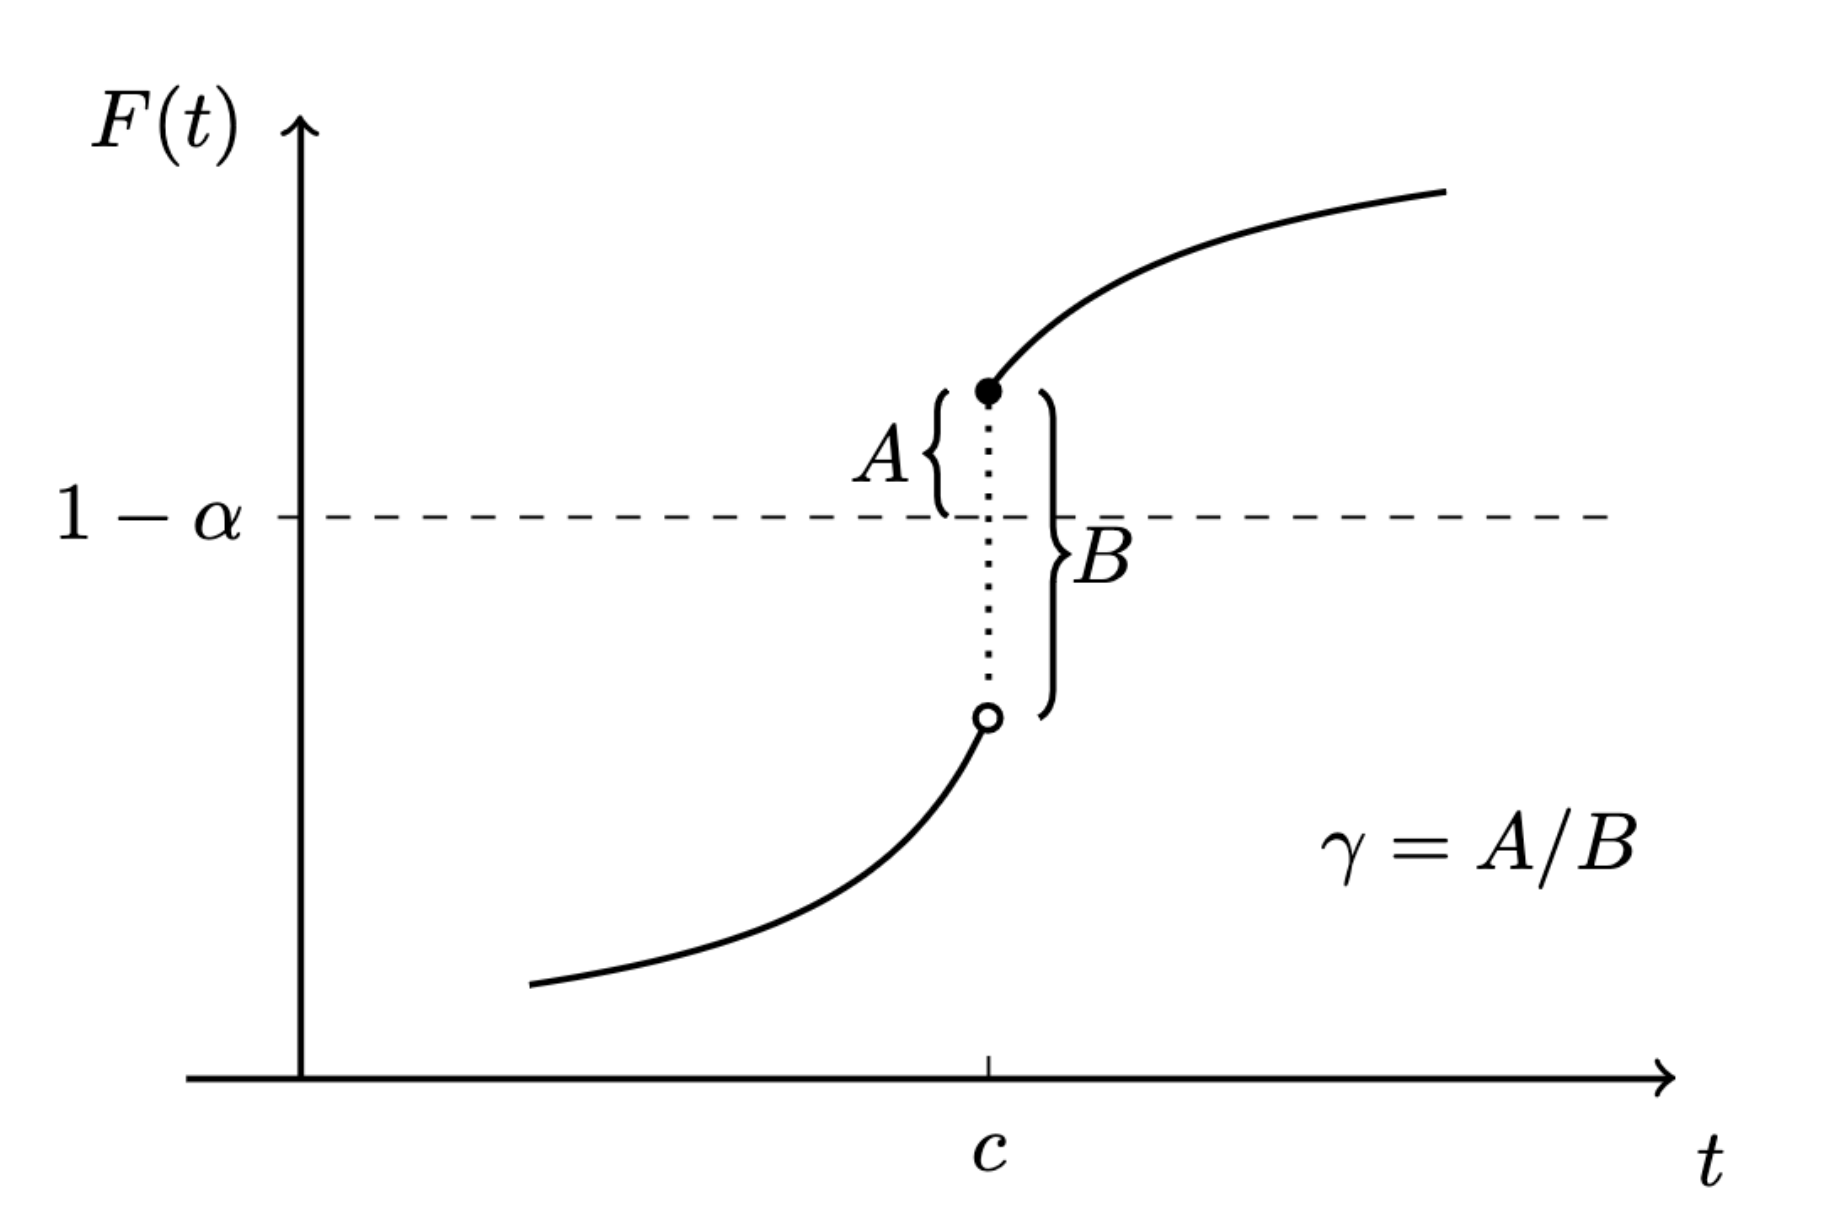
\includegraphics[width=0.8\textwidth]{./img/randomization_constant}
    \caption{Randomization constant}
    \label{fig:randomization_constant}
\end{figure}

\begin{ex}[Binomial Proportion]
    
Let $\bs{X} = (X_1, ..., X_n)$ be independent Bernoulli trials where $X_i \sim \text{Bern}(\theta)$. We observe the sequence of successes and failures.
Consider the simple hypotheses:
\[ H_0: \theta = \theta_0 \quad \text{vs.} \quad H_1: \theta = \theta_1, \quad \text{with } 0 < \theta_0 < \theta_1 < 1. \]

\subsubsection{Deriving the Test}
According to the Neyman-Pearson Lemma, the MP test rejects $H_0$ for large values of the likelihood ratio:
\[ \Lambda(\bs{x}) = \frac{p_{\theta_1}(\bs{x})}{p_{\theta_0}(\bs{x})} > k. \]

The likelihood for a binary sequence $\bs{x} \in \{0, 1\}^n$ is:
\[ p_\theta(\bs{x}) = \prod_{i=1}^n \theta^{x_i} (1-\theta)^{1-x_i} = \theta^{\sum x_i} (1-\theta)^{n - \sum x_i}. \]

Substituting this into the ratio:
\[
\frac{p_{\theta_1}(\bs{x})}{p_{\theta_0}(\bs{x})} 
= \frac{\theta_1^{\sum x_i} (1-\theta_1)^{n - \sum x_i}}{\theta_0^{\sum x_i} (1-\theta_0)^{n - \sum x_i}} 
= \left( \frac{\theta_1}{\theta_0} \cdot \frac{1-\theta_0}{1-\theta_1} \right)^{\sum\limits_{i=1}^n x_i} \left( \frac{1-\theta_1}{1-\theta_0} \right)^n.
\]

\paragraph{Simplification via Monotonicity}
The term $\left( \frac{1-\theta_1}{1-\theta_0} \right)^n$ is a constant (does not depend on data).
Because we assumed $\theta_1 > \theta_0$, the base of the exponent term is strictly greater than 1:
\[ \frac{\theta_1 (1-\theta_0)}{\theta_0 (1-\theta_1)} > 1. \]
Therefore, the likelihood ratio is a strictly \textbf{increasing function} of the sufficient statistic $T(\bs{x}) = \sum\limits_{i=1}^n X_i$.

Instead of defining a threshold $k$ on the likelihood ratio scale, we can define an equivalent threshold $c$ on the scale of $T(\bs{x})$. The test becomes:
\[
d(\bs{x}) = \begin{cases} 
1, & \text{if } T(\bs{x}) > c, \\ 
\gamma, & \text{if } T(\bs{x}) = c, \\ 
0, & \text{if } T(\bs{x}) < c. 
\end{cases}
\]

\subsubsection{Determining Constants $c$ and $\gamma$}
We need $\mathsf{E}_{\theta_0}[d(\bs{X})] = \alpha$. Under $H_0$, the statistic follows a Binomial distribution:
\[ T(\bs{X}) \sim \text{Bin}(n, \theta_0). \]

Since this distribution is discrete, there may not be a integer $c$ such that $\mathsf{P}(T > c) = \alpha$.


We choose $c$ as the $(1-\alpha)$-quantile of $\text{Bin}(n, \theta_0)$. Specifically:
\begin{enumerate}
    \item Find $c$ such that $\mathsf{P}_{\theta_0}(T > c) \le \alpha$ but $\mathsf{P}_{\theta_0}(T \ge c) > \alpha$.
    \item Set $\gamma$ to account for the difference:
    \[ \gamma = \frac{\alpha - \mathsf{P}_{\theta_0}(T > c)}{\mathsf{P}_{\theta_0}(T = c)}. \]
\end{enumerate}
In practice (e.g., in R), $c$ is found via \texttt{qbinom(1-alpha, n, theta0)}.
\end{ex}

\subsection{Always Some Power}
\label{sec:always_some_power}

We can prove that an optimal test is always strictly better than a naive guess, provided the distributions are distinct.

\begin{corollary}[Lehmann and Romano 2005, Corollary 3.2.1]
Let $\alpha \in (0,1)$, and let $d$ be a most powerful level $\alpha$ test for a simple vs. simple problem where $\mathsf{P}_{\theta_0} \neq \mathsf{P}_{\theta_1}$. Then the power $\beta$ satisfies:
\[ \beta = \mathsf{E}_{\theta_1}[d(X)] > \alpha \ge \mathsf{E}_{\theta_0}[d(X)]. \]
\end{corollary}

\begin{proof}
Consider a trivial competitor test $d^*(x) \equiv \alpha$ (the ``Three Monkeys" test: ignore data, reject with probability $\alpha$ regardless of observation).
\begin{itemize}
    \item The size of $d^*$ is $\mathsf{E}_{\theta_0}[d^*(X)] = \alpha$. Thus, $d^*$ is a valid level $\alpha$ test.
    \item The power of $d^*$ is $\mathsf{E}_{\theta_1}[d^*(X)] = \alpha$.
\end{itemize}

Since $d$ is the Most Powerful test, it must be at least as powerful as $d^*$. Thus $\beta \ge \alpha$.

\textbf{Proof of Strict Inequality (by contradiction):}
Assume $\beta = \alpha$. Then $d^*$ is also a Most Powerful test (it achieves the maximum power $\alpha$).
By the uniqueness part of the Neyman--Pearson Lemma (\autoref{thm:neyman_pearson}), any MP test must satisfy the form:
\[ d^*(x) = \begin{cases} 1 & p_1(x) > k p_0(x) \\ 0 & p_1(x) < k p_0(x) \end{cases} \quad \text{a.e.} \]
However, $d^*(x)$ is constantly $\alpha$ (never 0 or 1, assuming $\alpha \in (0,1)$).
This implies that we are almost always in the ``tie" case where $p_1(x) = k p_0(x)$.

Thus, $p_1(x) = k p_0(x)$ almost everywhere. Integrating both sides:
\[ \int p_1(x) d\nu = k \int p_0(x) d\nu \implies 1 = k(1) \implies k=1. \]
If $k=1$, then $p_1(x) = p_0(x)$ almost everywhere, which means $P_{\theta_1} = P_{\theta_0}$. This contradicts the assumption that the distributions are distinct.
Therefore, $\beta > \alpha$.
\end{proof}

\section{Uniformly Most Powerful Tests}
\label{sec:ump_tests}

In the previous section, we found the optimal test for a \textit{simple} alternative (e.g., $\theta = \theta_1$). Now we consider \textbf{composite} hypotheses, where the alternative hypothesis contains multiple distributions.

\[ H_0: \theta \in \Theta_0 \quad \text{vs.} \quad H_1: \theta \in \Theta_1 \]
where $|\Theta_1| > 1$.

\begin{definition}[Size and Level]
The \textbf{size} of a test $d$ is the maximum probability of Type I error over the null hypothesis space:
\[ \text{Size}(d) = \sup_{\theta \in \Theta_0} \mathsf{E}_{\theta}[d(X)]. \]
A test $d$ has \textbf{level} $\alpha$ if its size is at most $\alpha$.
\end{definition}

\begin{definition}[Uniformly Most Powerful]
Let $D(\alpha)$ be the set of all level $\alpha$ tests. A test $d \in D(\alpha)$ is a \textbf{Uniformly Most Powerful (UMP)} level $\alpha$ test if it is more powerful than any other level $\alpha$ test at \textit{every} point in the alternative hypothesis:
\[ \mathsf{E}_{\theta}[d(X)] \ge \mathsf{E}_{\theta}[d'(X)] \qquad \forall d' \in D(\alpha) \text{ and } \forall \theta \in \Theta_1. \]
\end{definition}



\begin{ex}[Binomial Proportion, One--Sided] 
    
Recall the Binomial example where $X_i \sim \text{Bin}(1, \theta) = \text{Bern}(\theta)$ and $T(X) = \sum\limits_{i=1}^{n} X_i$.
We have shown that the MP level \(\alpha\) test of 
\[
    H_0 \: : \: \theta = \theta_0 \text{ vs. } H_1 \: : \: \theta = \theta_1 \quad \text{ for }0<\theta_0<\theta_1<1
\]
is of the form 
\[
    d_{\theta_0,\theta_1,\alpha}(\bs{x}) = \bs{1}_{(c,\infty)}(T(\bs{x})) + \gamma \bs{1}_{\{c\}}(T(\bs{x})).
\]

Consider the composite alternative:
\[ H_0: \theta = \theta_0 \quad \text{vs.} \quad H_1: \theta > \theta_0. \]

From the Neyman-Pearson Lemma, for any \textit{specific} alternative $\theta_1 > \theta_0$, the Most Powerful (MP) test rejects for large values of $T(X)$:
\[ d_{\theta_0, \theta_1}(\mathbf{x}) = \begin{cases} 1 & \text{if } T(\mathbf{x}) > c \\ \gamma & \text{if } T(\mathbf{x}) = c \\ 0 & \text{if } T(\mathbf{x}) < c \end{cases} \]
where $c$ and $\gamma$ are determined by the equation $\mathsf{E}_{\theta_0}[d(X)] = \alpha$.

\paragraph{Key Observation:}
Notice that the constants $c$ and $\gamma$ depend \textbf{only} on the null distribution $\text{Bin}(n, \theta_0)$ and the significance level $\alpha$. They do \textbf{not} depend on the specific value of $\theta_1$, as long as $\theta_1 > \theta_0$ (which ensures the likelihood ratio is increasing in $T$).

\begin{quote}
\textit{Intuition:} If Student A tests $H_0: \theta=0.5$ vs $H_1: \theta=0.75$, and Student B tests $H_0: \theta=0.5$ vs $H_1: \theta=0.9$, they will derive the \textbf{exact same test} (same threshold $c$, same $\gamma$). Since this single test is optimal for every single $\theta > \theta_0$ individually, it is \textbf{Uniformly Most Powerful} for the entire set $\theta > \theta_0$.
\end{quote}

\subsubsection{Expanding the Null Hypothesis}

The test $d_{\theta_0}$ derived above is UMP for $H_0: \theta = \theta_0$ vs $H_1: \theta > \theta_0$.

Can we expand the null hypothesis to include all values less than $\theta_0$?
\[ H_0: \theta \le \theta_0 \quad \text{vs.} \quad H_1: \theta > \theta_0 \]

For the test to be valid for this expanded null, we must ensure its size is still $\alpha$. That is, the probability of rejection must not exceed $\alpha$ for any $\theta < \theta_0$.

This holds true because the power function $\beta(\theta) = \mathsf{E}_{\theta}[d(X)]$ is \textbf{monotonically increasing} in $\theta$.
\[ \beta(\theta) = \sum_{t=c+1}^{n} \binom{n}{t} \theta^t (1-\theta)^{n-t} + \gamma \binom{n}{c} \theta^c (1-\theta)^{n-c}. \]
One can show by differentiation that $\beta'(\theta) > 0$. Therefore:
\[ \sup_{\theta \le \theta_0} \beta(\theta) = \beta(\theta_0) = \alpha. \]

\textbf{Conclusion:}
The test $d_{\theta_0}$ is the UMP level $\alpha$ test for the one--sided problem $H_0: \theta \le \theta_0$ vs $H_1: \theta > \theta_0$.
\end{ex}

\section{Monotone Likelihood Ratio}
\label{sec:monotone_likelihood_ratio}

The Binomial example generalizes to a broader class of problems.
For $\theta_0, \theta_1 \in \Theta$, define the \textbf{likelihood ratio}:
\[
L_{\theta_1/\theta_0}(x) = \frac{p_{\theta_1}(x)}{p_{\theta_0}(x)} \cdot \mathbf{1}_{(0,\infty)}(p_{\theta_0}(x)) + \infty \cdot \mathbf{1}_{\{0\}}(p_{\theta_0}(x)),
\]
where $p_{\theta_0}$ and $p_{\theta_1}$ are densities of $\mathsf{P}_{\theta_0}$ and $\mathsf{P}_{\theta_1}$ with respect to a measure $\nu$.

\begin{definition}[Monotone Likelihood Ratio]
\label{def:mlr}
A one-parameter family $\{\mathsf{P}_{\theta}: \theta \in \Theta\}$ with $\Theta \subseteq \mathbb{R}$ has a \textbf{monotone likelihood ratio (MLR)} in a statistic $T: \mathcal{X} \to \mathbb{R}$ if for all $\theta_0 < \theta_1$:

\begin{enumerate}[label=\roman*)]
    \item $\mathsf{P}_{\theta_0} \neq \mathsf{P}_{\theta_1}$, and
    \item The likelihood ratio $L_{\theta_1/\theta_0}(x)$ is almost everywhere a non-decreasing function of $T(x)$. That is, there exists a non-decreasing function $H_{\theta_1/\theta_0}: \mathbb{R} \to [0, \infty]$ such that:
    \[ L_{\theta_1/\theta_0}(x) = H_{\theta_1/\theta_0}(T(x)) \]
    almost surely under both $\mathsf{P}_{\theta_0}$ and $\mathsf{P}_{\theta_1}$.
\end{enumerate}
\end{definition}



\begin{ex}[]
    
\label{sec:mlr_examples}

Many common statistical families satisfy the MLR property. Note that for i.i.d. observations, the relevant statistic $T(x)$ is often the sufficient statistic we are familiar with.

\begin{enumerate}
    \item \textbf{Binomial / Bernoulli:}
    \begin{itemize}
        \item $\{\bigotimes_{i=1}^{n} \text{Bin}(1,\theta) : \theta \in (0,1)\}$ has MLR in $T(x) = \sum\limits_{i=1}^{n} x_i$.
        \item $\{\text{Bin}(n,\theta) : \theta \in (0,1)\}$ has MLR in $T(x) = x$.
    \end{itemize}

    \item \textbf{Normal (Known Variance):}
    \[ \{\bigotimes_{i=1}^{n} \mathcal{N}(\theta, \sigma^{2}) : \theta \in \mathbb{R}\} \quad \text{has MLR in } T(x) = \overline{x}. \]
    
    \item \textbf{Hypergeometric:}
    \[ \{\text{Hypergeometric}(N, \theta, n) : \theta \in \{0, ..., n\}\} \quad \text{has MLR in } T(x) = x. \]

    \item \textbf{Poisson:}
    \[ \{\bigotimes_{i=1}^n \text{Poi}(\theta) : \theta > 0\} \quad \text{has MLR in } T(x) = \sum_{i=1}^n x_i. \]

    \item \textbf{Uniform (Continuous):}
    \[ \{\bigotimes_{i=1}^n \text{Uniform}(0,\theta) : \theta > 0\} \quad \text{has MLR in } T(x) = \max_{1 \le i \le n} x_i. \]
    \begin{remark}[]
    This is not an exponential family, but it still possesses MLR.
    \end{remark}

    \item \textbf{Advanced Distributions:}
    Further examples include noncentral $\chi^2$, noncentral $F$, or noncentral $t$-distributions (often parameterized by a non-centrality parameter).
\end{enumerate}
\end{ex}

\subsubsection{Counter-Example: The Cauchy Distribution}
The \textbf{Cauchy location family} defined by the density:
\[ p_{\theta}(x) = \frac{1}{\pi} \cdot \frac{1}{1 + (x - \theta)^2}, \quad \theta \in \mathbb{R}, \]
does \textbf{not} have a Monotone Likelihood Ratio in $x$ (or in any other statistic $T(x)$).

\textit{Why?} Although shifting the center of a Cauchy distribution increases the probability of values near the new center, the heavy tails mean that extremely large values of $x$ do not necessarily provide stronger evidence for the larger $\theta$, causing the likelihood ratio to oscillate or decrease eventually.

\subsection{Exponential Families and MLR}
\label{sec:exponential_families_mlr}

One-parameter exponential families provide a powerful source of models with the Monotone Likelihood Ratio property.

\begin{pro}
\label{prop:exp_family_mlr}
If $\{\mathsf{P}_{\theta} : \theta \in \Theta\}$ with $\Theta \subseteq \mathbb{R}$ forms a one-parameter exponential family with densities:
\[
p_{\theta}(x) = c(\theta) \cdot \exp\{\eta(\theta) T(x)\} \cdot h(x), \quad x \in \mathcal{X},
\]
and the natural parameter $\eta(\theta)$ is a \textbf{strictly increasing} function of $\theta$, then the family has MLR in the sufficient statistic $T(x)$.
\end{pro}

\begin{proof}
Let $\theta_1 > \theta_0$. The likelihood ratio is:
\[
L_{\theta_1/\theta_0}(x) = \frac{p_{\theta_1}(x)}{p_{\theta_0}(x)} 
= \frac{c(\theta_1) e^{\eta(\theta_1) T(x)} h(x)}{c(\theta_0) e^{\eta(\theta_0) T(x)} h(x)}
= \frac{c(\theta_1)}{c(\theta_0)} \exp\left\{ [\eta(\theta_1) - \eta(\theta_0)] \cdot T(x) \right\}.
\]
Since $\eta$ is strictly increasing, $[\eta(\theta_1) - \eta(\theta_0)] > 0$. 
The function $y \mapsto e^{ay}$ with $a>0$ is increasing. Therefore, $L_{\theta_1/\theta_0}(x)$ is an increasing function of $T(x)$.
\end{proof}

\begin{ex}[Gaussian Mean]
    
\label{ex:gaussian_mean_ump}

Let $X_1, ..., X_n \stackrel{\text{iid}}{\sim} \mathcal{N}(\theta, \sigma^2)$ with $\theta \in \mathbb{R}$ unknown and $\sigma^2$ known.
We wish to test:
\[ H_0: \theta \le \theta_0 \quad \text{vs.} \quad H_1: \theta > \theta_0. \]

\subsubsection{Checking MLR}
First, we verify the MLR property. For any $\theta_1 > \theta_0$, the likelihood ratio is:
\[
\begin{split} 
L_{\theta_1/\theta_0}(\bs{x}) &= \frac{\prod\limits_{i=1}^n \exp\left\{\frac{-1}{2\sigma^2} (x_i - \theta_1)^2\right\}}{\prod\limits_{i=1}^n \exp\left\{\frac{-1}{2\sigma^2} (x_i - \theta_0)^2\right\}} \quad (\text{constants cancel}) \\ 
&= \exp\left\{-\frac{1}{2\sigma^2} \sum_{i=1}^n \left[(x_i - \theta_1)^2 - (x_i - \theta_0)^2\right]\right\} \\
&= \exp\left\{-\frac{1}{2\sigma^2} \sum_{i=1}^n \left[ x_i^2 - 2x_i\theta_1 + \theta_1^2 - (x_i^2 - 2x_i\theta_0 + \theta_0^2) \right] \right\} \\
&= \exp\left\{-\frac{1}{2\sigma^2} \left[ 2(\theta_0 - \theta_1)\sum\limits_{i=1}^{n}  x_i + n(\theta_1^2 - \theta_0^2) \right] \right\} \\
&= \exp\left\{ \frac{n(\theta_1 - \theta_0)}{\sigma^2} \overline{x}_n \right\} \cdot C(\theta_0, \theta_1).
\end{split}
\]
Since $\theta_1 > \theta_0$, the coefficient of $\overline{x}_n$ is positive. Thus, the family has MLR in $T(\bs{x}) = \overline{x}_n$.

\subsubsection{The UMP Test}
Since the family has MLR in $\overline{x}_n$, the UMP level $\alpha$ test rejects for large values of $\overline{x}_n$:
\[
d(\bs{x}) = \begin{cases} 
1, & \text{if } \overline{x}_n \ge c, \\ 
0, & \text{if } \overline{x}_n < c. 
\end{cases}
\]
\begin{remark}[]
 Since the distribution is continuous, $\mathsf{P}(\overline{x}_n = c) = 0$, so the randomization constant $\gamma$ is irrelevant and we can simply reject at equality.
\end{remark}

\textbf{Determining $c$:}
We require size $\alpha$ at the boundary $\theta_0$:
\[ \mathsf{P}_{\theta_0}(\overline{X}_n \ge c) = \alpha. \]
Under $\theta_0$, $\overline{X}_n \sim \mathcal{N}(\theta_0, \sigma^2/n)$. Standardizing:
\[ \mathsf{P}\left( \frac{\overline{X}_n - \theta_0}{\sigma/\sqrt{n}} \ge \frac{c - \theta_0}{\sigma/\sqrt{n}} \right) = \alpha \implies \frac{c - \theta_0}{\sigma/\sqrt{n}} = z_{1-\alpha}. \]
Thus, $c = \theta_0 + z_{1-\alpha} \frac{\sigma}{\sqrt{n}}$.



\subsubsection{Expanding the Null Hypothesis}
This test is derived for $H_0: \theta = \theta_0$.
Is it valid for $H_0: \theta \le \theta_0$?

Yes, because the power function $\beta(\theta) = \mathsf{P}_\theta(\text{Reject})$ is strictly increasing.

\textbf{Proof of Monotonicity:}
Let $\theta < \tilde{\theta}$. We use the fact that if $Z \sim \mathcal{N}(0, \sigma^2/n)$, then $\overline{X}_n \stackrel{d}{=} Z + \theta$.
\[
\begin{split} 
\beta(\theta) &= \mathsf{P}_{\theta}(\overline{X}_n > c) \\
&= \mathsf{P}(Z + \theta > c) \\
&= \mathsf{P}(Z > c - \theta).
\end{split}
\]
Since $\theta < \tilde{\theta}$, we have $c - \theta > c - \tilde{\theta}$.
Therefore, $\mathsf{P}(Z > c - \theta) < \mathsf{P}(Z > c - \tilde{\theta})$, which implies $\beta(\theta) < \beta(\tilde{\theta})$.

Since the power is increasing, $\sup\limits_{\theta \le \theta_0} \beta(\theta) = \beta(\theta_0) = \alpha$. The test is valid and UMP for the composite null.
\end{ex}

\subsection{UMP Tests and Monotone Likelihood Ratios}
\label{sec:ump_mlr_theorem}

We can now formalize the generalization of the Binomial and Gaussian examples into a powerful theorem.

\begin{theo}[Lehmann and Romano 2005, Thm 3.4.1]
\label{thm:ump_mlr}
Suppose $\{\mathsf{P}_{\theta}: \theta \in \Theta\}$, $\Theta \subseteq \mathbb{R}$, has \textbf{Monotone Likelihood Ratio (MLR)} in $T(x)$. Let $\theta_0 \in \Theta$ and $\alpha \in (0,1)$.
Consider the test $d(x)$ defined by:
\[
d(x) = \begin{cases} 
1, & \text{if } T(x) > c, \\ 
\gamma, & \text{if } T(x) = c, \\ 
0, & \text{if } T(x) < c, 
\end{cases}
\]
where $c \in \mathbb{R}$ and $\gamma \in [0,1]$ are chosen such that $\mathsf{E}_{\theta_0}[d(X)] = \alpha$ (i.e., size is exactly $\alpha$ at the boundary).

Then the following properties hold:

\begin{enumerate}[label=\roman*)]
    \item \textbf{UMP Property:} The test $d$ is the Uniformly Most Powerful (UMP) level $\alpha$ test for:
    \[ H_0: \theta \leq \theta_0 \quad \text{vs.} \quad H_1: \theta > \theta_0. \]
    
    \item \textbf{Monotonicity:} The power function $\beta(\theta) = \mathsf{E}_{\theta}[d(X)]$ is non-decreasing. It is strictly increasing for all $\theta$ where $0 < \beta(\theta) < 1$.
    
    \item \textbf{Minimizing Error under Null:} For all $\theta \le \theta_0$, the test minimizes the probability of Type I error among all tests that have size $\alpha$ at the boundary:
    \[ \beta(\theta) = \min \{ \mathsf{E}_{\theta}[\tilde{d}] : \tilde{d} \text{ is a test with } \mathsf{E}_{\theta_0}[\tilde{d}] = \alpha \}. \]
\end{enumerate}
\end{theo}

\begin{proof}[]
    \leavevmode
        \begin{enumerate}[label=\roman*)]
            \item 
This follows directly from the Neyman-Pearson Lemma and the definition of MLR.
\begin{enumerate}[label=\arabic*.]
\item  Pick any specific alternative $\theta_1 > \theta_0$.
\item  The NP Lemma says the MP test rejects when the likelihood ratio $L_{\theta_1/\theta_0}(x)$ is large.
\item Since the family has MLR, $L_{\theta_1/\theta_0}(x)$ is increasing in $T(x)$. Therefore, ``large likelihood ratio" is equivalent to ``$T(x) > c$".
\item  Since this test form depends only on the direction ($\theta > \theta_0$) and not the specific value $\theta_1$, it is optimal for \textit{all} $\theta > \theta_0$ simultaneously.
\end{enumerate}

\item 
The power function must be increasing. If we treat $\theta'$ as a null and $\theta''$ as an alternative (where $\theta' < \theta''$), the test $d$ is Most Powerful. By the corollary ``MP tests always have power $\ge$ size," we must have $\beta(\theta'') \ge \beta(\theta')$. This ensures that testing $H_0: \theta \le \theta_0$ is valid, because the maximum error rate (size) occurs at the boundary $\theta_0$.

\item 
This part is proven by a ``flipping" argument.
Consider the test $1-d(x)$, which rejects when $T(x)$ is \textit{small}. This corresponds to testing the reverse hypothesis (e.g., $H_0: \theta = \theta_0$ vs $H_1: \theta < \theta_0$).
Since $d$ maximizes power for $\theta > \theta_0$, the test $1-d$ maximizes power for $\theta < \theta_0$ (relative to the reverse problem).
Maximizing $\mathsf{E}[1-d]$ is equivalent to minimizing $\mathsf{E}[d]$. Therefore, for $\theta < \theta_0$, our original test $d$ has the minimal possible rejection probability.

\begin{note}
This means not only is the test good at rejecting the null when it's false (power), but it is also the best at accepting the null when it is true (minimizing Type I error) compared to any other test that spends the same error budget $\alpha$ at the boundary $\theta_0$.
\end{note}
        \end{enumerate}
\end{proof}

\section{Discussion of Two-Sided Testing Problems}
\label{sec:two_sided_testing}

Consider the standard two-sided testing problem:
\[ H_0: \theta = \theta_0 \quad \text{vs.} \quad H_1: \theta \neq \theta_0 \]

\subsubsection{Non-Existence of UMP Tests}
Typically, a Uniformly Most Powerful (UMP) test \textbf{does not exist} for this problem.

\textbf{Why?}
To be UMP for the two-sided alternative, a test $d$ would need to have a power function $\beta_d(\theta)$ that is at least as high as \textit{any} other level $\alpha$ test for \textit{every} $\theta \neq \theta_0$.
\begin{itemize}
    \item There exists a UMP test $d_1$ for $H_1: \theta > \theta_0$ (high power on the right, low on the left).
    \item There exists a UMP test $d_2$ for $H_1: \theta < \theta_0$ (high power on the left, low on the right).
\end{itemize}
A hypothetical two-sided UMP test would need to match the power of $d_1$ on the right and $d_2$ on the left. This would require the power function to be extremely high on both sides while instantaneously dropping to $\alpha$ at exactly $\theta_0$. Due to the smoothness of power functions (especially in exponential families), such a function usually cannot exist without violating the level constraint.

\subsubsection{The Solution: Unbiasedness}
Since we cannot satisfy the UMP condition everywhere, we restrict our search to a smaller, more ``reasonable" class of tests: \textbf{Unbiased Tests}.

\begin{definition}[Unbiased Test]
A test with power function $\beta(\theta)$ is \textbf{unbiased} at level $\alpha$ if:
\begin{align*}
    \beta(\theta) &\le \alpha \quad \forall \theta \in \Theta_0 \quad \text{(Control Type I Error)} \\
    \beta(\theta) &\ge \alpha \quad \forall \theta \in \Theta_1 \quad \text{(Power never worse than random guessing)}
\end{align*}
\end{definition}

By restricting the competition to unbiased tests, we can often find a \textbf{Uniformly Most Powerful Unbiased (UMPU)} test.
\begin{itemize}
    \item For the Normal mean (variance known), the UMPU test rejects when $| \overline{x} - \theta_0 |$ is large.
    \item This corresponds to symmetric rejection regions (e.g., using $\alpha/2$ on both tails).
\end{itemize}

\section{\(p\)--Values}
\label{sec:p_values}

In practice, data analysis often requires checking multiple significance levels or reporting the strength of evidence rather than a simple ``Yes/No" decision.

%\subsection{Definition and Calculation}

Suppose we have a family of non-randomized tests $d_\alpha$ for every level $\alpha \in (0,1)$ with \textbf{nested rejection regions} (i.e., rejecting at a smaller $\alpha$ implies rejecting at a larger $\alpha$).

\begin{definition}[\(p\)--value]
The \textbf{\(p\)--value} $p(x)$ is the smallest significance level at which the observed data leads to rejection:
\[ 
p(x) = \inf \{ \alpha \in (0,1) : d_\alpha(x) = 1 \}.
\]
\end{definition}

For standard tests that reject for large values of a statistic $T(X)$, the \(p\)--value corresponds to the probability of observing a statistic as extreme or \textit{more extreme} than the observed value $T(x_{obs})$ under the null hypothesis:

\[ 
p(x_{obs}) = \sup_{\theta \in \Theta_0} \mathsf{P}_{\theta} \left( T(X) \ge T(x_{obs}) \right). 
\]

If the null distribution is unique (e.g., $T(X) \sim \mathcal{N}(0,1)$ under $H_0$), this simplifies to:
\[ 
p(x_{obs}) = \mathsf{P}_0(T(X) \ge T(x_{obs})). 
\]

\subsubsection{Practical Interpretation}

The \(p\)--value serves as a continuous measure of evidence against the null hypothesis.

\begin{itemize}
    \item \textbf{Small \(p\)--value (e.g., $< 0.05$):} Strong evidence \textit{against} $H_0$. 
    \item \textbf{Large \(p\)--value:} No evidence against $H_0$. 
        \begin{remark}[]
        This does \textbf{not} prove $H_0$ is true; it merely indicates the data is consistent with it.
        \end{remark}
\end{itemize}

\paragraph{The ``Lottery" Analogy:}
If you observe a very small \(p\)--value (e.g., $p = 0.0001$), you are faced with two possibilities:
\begin{enumerate}[label=\alph*)]
    \item The null hypothesis is true, and you have just witnessed a highly improbable ``lottery win" event.
    \item The null hypothesis is false.
\end{enumerate}
Scientific testing generally proceeds by betting on the second option.

\subsubsection{Decision Rule}
If a specific significance level $\alpha_{\text{target}}$ is fixed in advance, the decision rule using the \(p\)--value is:

\[
\text{Decision} = \begin{cases} 
\text{Reject } H_0 & \text{if } p(x) \le \alpha_{\text{target}}, \\
\text{Do not reject } H_0 & \text{if } p(x) > \alpha_{\text{target}}.
\end{cases}
\]

\subsection{Uniformity of \(p\)--Values}
\label{sec:uniformity_p_values}

A crucial property of \(p\)--values is their behavior when the null hypothesis is actually true. Understanding this helps distinguish genuine signals from random noise.

Informally: \textbf{Under the null hypothesis, the \(p\)--value is uniformly distributed on $(0,1)$.}

This means that if $H_0$ is true (e.g., ``red wine has no effect on health") and you repeat the experiment many times, you are equally likely to get a \(p\)--value of 0.01, 0.45, or 0.99.
\begin{itemize}
    \item \textbf{Under $H_0$:} The histogram of \(p\)--values is flat.
    \item \textbf{Under $H_1$:} The histogram of \(p\)--values spikes near 0 (small \(p\)--values are more likely).
\end{itemize}

\begin{lemma}[Lehmann and Romano 2005, Lemma 3.3.1).]
Suppose $X \sim \mathsf{P}_{\theta}$ with $\theta \in \Theta_0$ (the null is true).

\begin{enumerate}
    \item[(i)] If the test size is controlled for all levels, i.e.,
    \[ \sup_{\theta \in \Theta_0} \mathsf{P}_{\theta}(d_{\alpha}(X) = 1) \leq \alpha \qquad \forall \alpha \in (0,1), \]
    then the \(p\)--value is \textbf{stochastically larger} than the Uniform(0,1) distribution:
    \[ \mathsf{P}_{\theta}(p(X) \le u) \le u \quad \forall u \in [0, 1]. \]

    \item[(ii)] If the test size is \textit{exactly} equal to $\alpha$ for all levels, i.e.,
    \[ \mathsf{P}_{\theta}(d_{\alpha}(X) = 1) = \alpha \qquad \forall \alpha \in (0, 1), \]
    then:
    \[ p(X) \sim \text{Unif}(0, 1). \]
\end{enumerate}
\end{lemma}

\begin{proof}
    \leavevmode
        \begin{enumerate}[label=\roman*)]
            \item 
By the definition of the \(p\)--value ($p(x) = \inf\{\alpha : d_\alpha(x)=1\}$) and the nested rejection regions assumption:
If $p(x) \le u$, then for any significance level $\nu > u$, the test must reject ($d_\nu(x) = 1$).
Therefore, for any $\nu > u$:
\[ \{ x : p(x) \le u \} \subseteq \{ x : d_\nu(x) = 1 \}. \]
Taking probabilities under $\theta \in \Theta_0$:
\[ \mathsf{P}_{\theta}(p(X) \le u) \le \mathsf{P}_{\theta}(d_{\nu}(X) = 1) \le \nu. \]
Since this holds for all $\nu > u$, we take the limit as $\nu \downarrow u$:
\[ \mathsf{P}_{\theta}(p(X) \le u) \le u. \]

\item 
Conversely, if a test rejects at level $u$ ($d_u(x) = 1$), then by definition the \(p\)--value must be less than or equal to $u$:
\[ \{ x : d_u(x) = 1 \} \subseteq \{ x : p(x) \le u \}. \]
Taking probabilities:
\[ \mathsf{P}_{\theta}(p(X) \le u) \ge \mathsf{P}_{\theta}(d_u(X) = 1) = u. \]
Combining the results from (i) and (ii) (since $\le u$ and $\ge u$ implies $= u$), we get:
\[ \mathsf{P}_{\theta}(p(X) \le u) = u. \]
This is the CDF of a Uniform(0,1) random variable.
        \end{enumerate}
\end{proof}

\subsubsection{Connection to Probability Integral Transform}
This result is related to the Probability Integral Transform. For a continuous random variable $T$ with CDF $F_T$, the random variable $Y = F_T(T)$ is uniformly distributed.
Since a one--sided \(p\)--value is essentially $1 - F_T(T(X))$ (calculating the tail area), it follows the same uniform distribution logic under the null.

\section{Confidence Sets}
\label{sec:confidence_sets}

\paragraph{Setup}
We consider the standard statistical setup:
\begin{itemize}
    \item Observation $X$ in sample space $\mathcal{X} \subset \mathbb{R}^d$.
    \item Statistical model $\mathcal{P}$ for the distribution of $X$.
    \item Target parameter $\gamma: \mathcal{P} \to \Gamma$ (e.g., the mean).
    \item Significance level $\alpha \in (0, 1)$, representing our ``budget for mistakes."
\end{itemize}

\medskip

\begin{definition}[Confidence Set]
A family of subsets $S(x)$ is a \textbf{confidence set of confidence level $1-\alpha$} if the probability that the random set covers the true parameter is at least $1-\alpha$ for all distributions in the model:
\[
\inf_{\mathsf{P}\in\mathcal{P}}\mathsf{P}(\gamma(\mathsf{P})\in S(X)) \geq 1-\alpha.
\]
The probability $\mathsf{P}(\gamma(\mathsf{P}) \in S(X))$ is called the \textbf{coverage probability}.
\end{definition}

\begin{ex}[Normal Mean]
    
Let $\bs{X} = (X_1, ..., X_n)$ be i.i.d. $\mathcal{N}(\mu, \sigma^2)$. The target parameter is the mean $\mu$.

\begin{figure}[htpb]
    \centering
    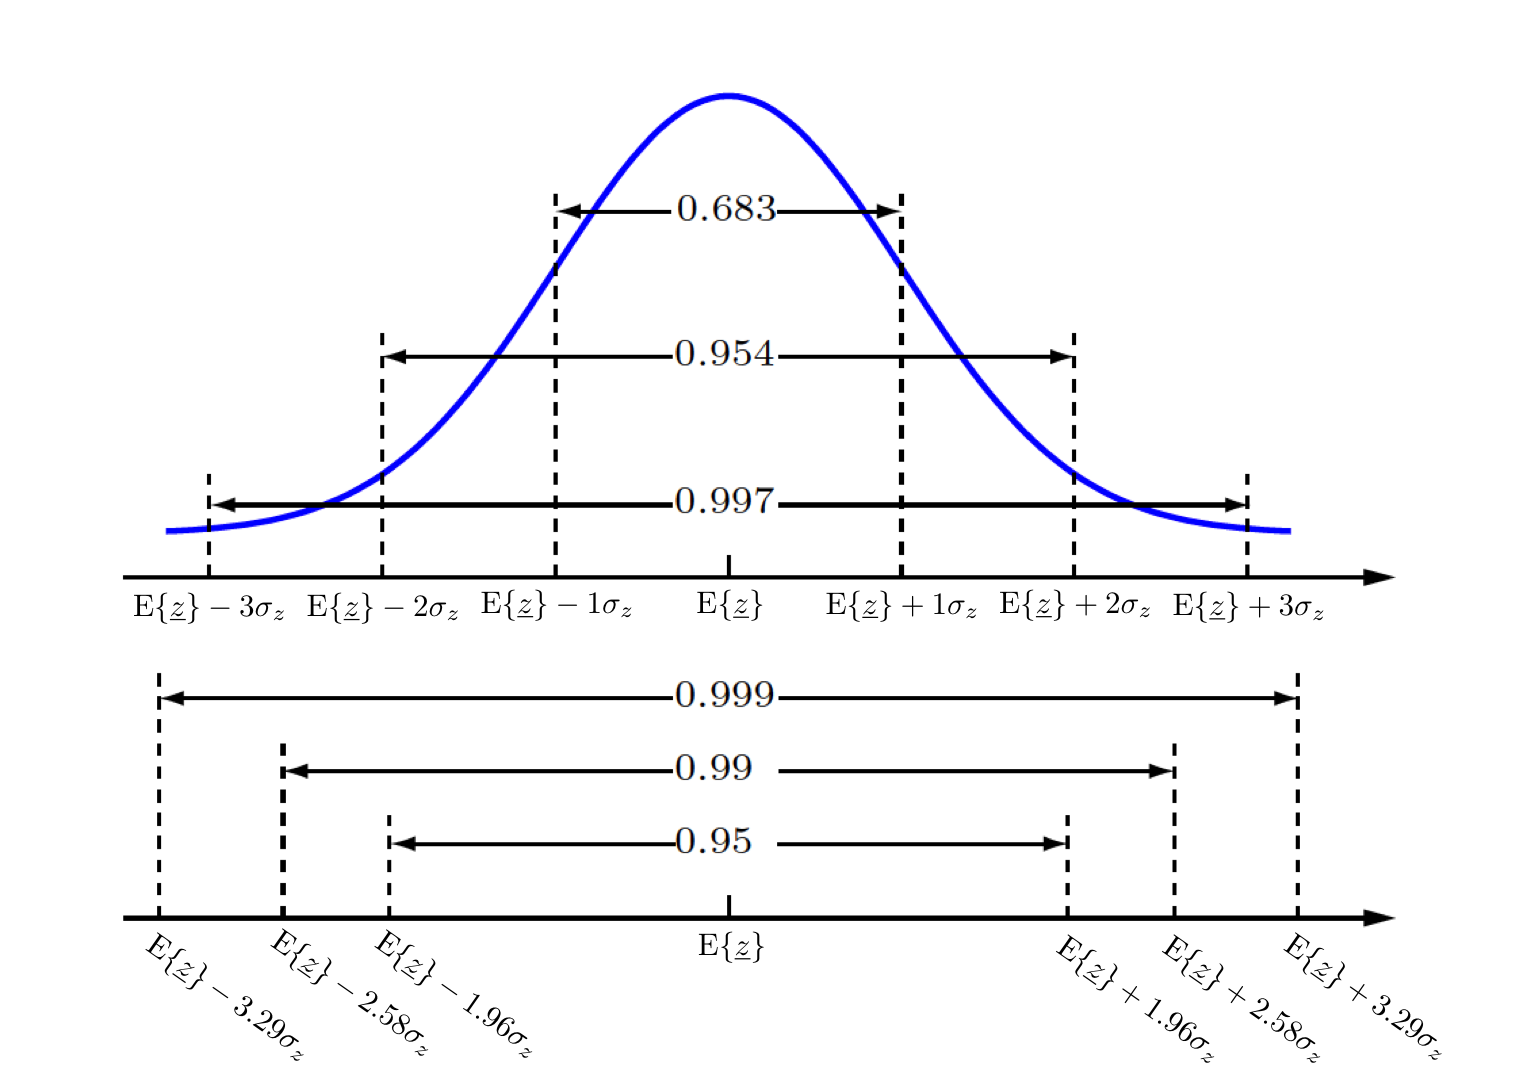
\includegraphics[width=0.8\textwidth]{./img/normal_cofidence_intervals}
    \caption{Standard normal distribution confidence interval}
    \label{fig:normal_confidence_intervals}
\end{figure}

    \begin{enumerate}[label=\alph*)]
        \item 
\textbf{Variance $\sigma^2 = \sigma_0^2$ is Known:}
When the variance is known, we use the quantiles of the standard normal distribution $\mathcal{N}(0,1)$. The $(1-\alpha)$ confidence interval is:

\[
S(\mathbf{x}) = \left(\overline{x}_n - z_{\alpha/2} \frac{\sigma_0}{\sqrt{n}}, \quad \overline{x}_n + z_{\alpha/2} \frac{\sigma_0}{\sqrt{n}}\right)
\]

where $z_{\alpha/2}$ is the $(1-\alpha/2)$-quantile of $\mathcal{N}(0,1)$.

\textbf{Derivation via Pivot:}
The construction relies on the random variable:
\[
Z = \frac{\overline{X}_n - \mu}{\sigma_0 / \sqrt{n}} \sim \mathcal{N}(0, 1)
\]
This variable $Z$ is a \textbf{pivot}: it depends on the data and the parameter, but its distribution (Standard Normal) is known and fixed. We construct the interval by requiring:
\[
\mathsf{P}\left( -z_{\alpha/2} \le \frac{\overline{X}_n - \mu}{\sigma_0/\sqrt{n}} \le z_{\alpha/2} \right) = 1 - \alpha
\]
Rearranging the inequalities to isolate $\mu$ yields the interval above.

\item 
\textbf{Variance $\sigma^2$ is Unknown:}
If $\sigma^2$ is unknown, we must estimate it using the sample standard deviation $s(\bs{x})$. We replace the normal quantile $z_{\alpha/2}$ with the quantile from the Student's $t$-distribution.

\[
S(\bs{x}) = \left(\overline{x}_n - t_{\alpha/2}(n-1)\frac{s(\bs{x})}{\sqrt{n}}, \quad \overline{x}_n + t_{\alpha/2}(n-1)\frac{s(\bs{x})}{\sqrt{n}}\right)
\]

\begin{itemize}
    \item $s(\bs{x}) = \sqrt{\frac{1}{n-1} \sum (x_i - \overline{x}_n)^2}$
    \item $t_{\alpha/2}(n-1)$ is the $(1-\alpha/2)$-quantile of the $t$-distribution with $n-1$ degrees of freedom.
    \item \textbf{Pivot:} $\frac{\overline{X}_n - \mu}{s(\bs{X})/\sqrt{n}} \sim t(n-1)$.
\end{itemize}

\item 
\textbf{One--Sided Intervals}
We can also form upper or lower confidence bounds (e.g., ``The mean is at least $L$").
\[
\text{Lower Bound: } \left(-\infty, \quad \overline{x}_n + t_{\alpha}(n-1)\frac{s(\bs{x})}{\sqrt{n}}\right)
\]
\[
\text{Upper Bound: } \left(\overline{x}_n - t_{\alpha}(n-1)\frac{s(\bs{x})}{\sqrt{n}}, \quad \infty\right)
\]
Note the use of $t_{\alpha}$ (all error budget on one side) rather than $t_{\alpha/2}$.
    \end{enumerate}
\end{ex}

\subsection{Pivots}

A \textbf{pivot} is a random variable that depends on the data and the parameter of interest, but whose probability distribution does \textit{not} depend on any unknown parameters.

\begin{definition}[Pivot]
A function $V: \mathcal{P} \times \mathcal{X} \to \mathbb{R}$ is a \textbf{pivot} for parameter $\gamma$ if:
\begin{enumerate}[label=\roman*)]
    \item $V(\mathsf{P}, X) = U(\gamma(\mathsf{P}), X)$ for some function $U \: : \: \Gamma \times \cc{X}\to \R$. (It depends on the underlying distribution only through the parameter of interest).
    \item For all $\mathsf{P}_1, \mathsf{P}_2 \in \mathcal{P}$, the distribution of $V(\mathsf{P}_1, X)$ is the same as $V(\mathsf{P}_2, X)$. (The distribution is fixed/known).
\end{enumerate}
\end{definition}

\textbf{Examples:}
\begin{itemize}
    \item \textbf{Z-Statistic (Known Variance):}
    \[ V = \frac{\overline{X}_n - \mu}{\sigma_0 / \sqrt{n}} \sim \mathcal{N}(0, 1). \]
    \item \textbf{T-Statistic (Unknown Variance):}
    \[ V = \frac{\overline{X}_n - \mu}{s(X)/\sqrt{n}} \sim t(n-1). \]
\end{itemize}

\subsubsection{Constructing Confidence Sets Using Pivots}
If $V$ is a pivot, we can construct a confidence set by ``inverting" the probability statement.
\begin{enumerate}
    \item Choose a set $A$ (based on the known distribution of $V$) such that:
    \[ \mathsf{P}(V(P, X) \in A) \ge 1 - \alpha. \]
    \item Define the confidence set $S(x)$ as the set of all parameter values that keep the pivot inside $A$:
    \[ S(x) = \{ \gamma(P) : V(P, x) \in A \}. \]
\end{enumerate}

\subsection{Duality: Confidence Sets and Hypothesis Tests}

There is a fundamental equivalence between confidence sets and hypothesis tests. You can convert one into the other.

\subsubsection{1. Confidence Sets $\to$ Tests}
If $S(x)$ is a $(1-\alpha)$ confidence set, we can define a level $\alpha$ test for $H_0: \gamma(P) = \gamma_0$ as:
\[
d_{\gamma_0}(x) = \begin{cases} 
1 (\text{Reject}) & \text{if } \gamma_0 \notin S(x), \\ 
0 (\text{Accept}) & \text{if } \gamma_0 \in S(x). 
\end{cases}
\]
\textit{Intuition:} If the hypothesized value $\gamma_0$ is not inside the ``plausible range" (the confidence set), we reject it.

\subsubsection{2. Tests $\to$ Confidence Sets (Test Inversion)}
If we have a family of level $\alpha$ tests $d_{\gamma_0}$ for every possible parameter value $\gamma_0$, we can build a confidence set by collecting all the values we do \textbf{not} reject:
\[
S(x) = \{ \gamma_0 \in \Gamma : d_{\gamma_0}(x) = 0 \}.
\]
The coverage probability is guaranteed:
\[
\mathsf{P}(\gamma(\mathsf{P}) \in S(X)) = \mathsf{P}(d_{\gamma(\mathsf{P})}(X) = 0) \ge 1 - \alpha.
\]
